\documentclass[main.tex]{subfiles} % Subfile-Class

% ============================================================================== %
%                            Subfile document                                    %
% ============================================================================== %

\begin{document}

% Template

\subsection{Aufgabenstellung}

Die Aufgabenstellung des Moduls Produktentwicklung PREN 1 der
Hochschule Luzern fordert das interdisziplinäre Team heraus, ein autonomes 
Fahrzeug zu entwickeln, das ein vorgegebenes Wegenetzwerk optimal navigieren kann. 
Das Fahrzeug soll Hindernisse erkennen, gesperrte Bereiche meiden und die kürzeste 
Route zum Ziel unter Berücksichtigung unbekannter Einschränkungen finden.

Das Team, das sich aus Studierenden der Fachrichtung Elektrotechnik, Informatik und Maschinenbau 
zusammensetzt, vereint ein breites Spektrum an technischen Kompetenzen. Im Rahmen der Projektphase von PREN 1 
erfolgt die Entwicklung eines Gesamtkonzepts, das auf einem morphologischen Kasten basiert. 
Ziel dieser Vorgehensweise ist der systematische Vergleich von Lösungsvarianten. Zunächst wird die technische
Machbarkeit bewertet, woraufhin erste Prototypen erstellt werden, die als Grundlage für das Modul PREN 2 dienen.

Zu den wichtigsten Anforderungen zählen:
\begin{itemize}
    \item \textbf{Erkennung gesperrter Wegpunkte:} Pylonen müssen selbstständig detektiert werden.
    \item \textbf{Bewältigung von Hindernissen:} Hindernisse sollen aktiv entfernt und zurückgestellt werden.
    \item \textbf{Anpassung an veränderte Bedingungen:} Fehlende Streckenabschnitte müssen als nicht passierbar erkannt werden.
    \item \textbf{Autonome Zielfindung:} Über eine Zielauswahl vor dem Start soll das Fahrzeug die effizienteste Route finden.
\end{itemize}

Zudem werden bei der Umsetzung strenge Vorgaben zu Dimensionen, Gewicht und
Autonomie des Systems berücksichtigt. Dies umfasst die Integration sämtlicher
Hardware-Komponenten des Fahrzeugs sowie die Sicherstellung eines
störungsfreien und sicheren Betriebs. Weiterhin wird in PREN 1 erste
Simulationen erarbeitet, die das Verhalten des Systems unter realitätsnahen Bedingungen
analysieren und optimieren.

Die wissenschaftliche Herausforderung besteht darin, Sensorik, Elektronik 
und Algorithmen so zu kombinieren, dass eine zuverlässige Wegfindung und 
Hindernisbewältigung gewährleistet ist. Dabei liegt ein besonderes Augenmerk auf 
eine methodische Herangehensweise, die auch Nachhaltigkeitsaspekte berücksichtigt.

Das Projekt bietet die Möglichkeit, theoretisches Wissen praktisch 
anzuwenden und die Kompetenzen in interdisziplinärer Zusammenarbeit 
und systematischer Produktentwicklung zu vertiefen.

\begin{figure}[H]
    \centering
    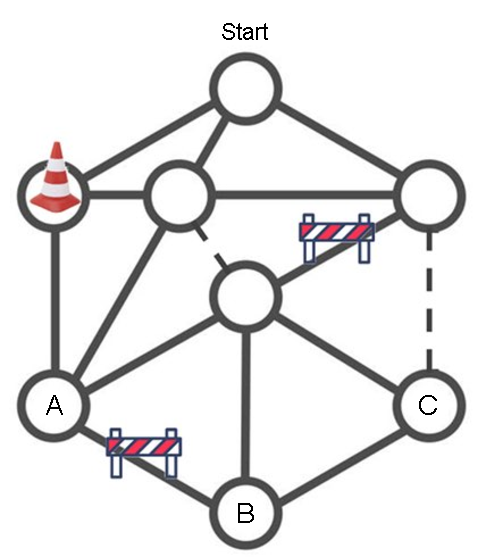
\includegraphics[width=0.25\textwidth]{Wegenetzwerk_Aufgabenstellung.pdf}
    \caption{Beispiel Wegenetzwerk aus Aufgabenstellung}~\label{fig:Wegenetzwerk_Aufgabenstellung}
\end{figure}

\end{document}